\documentclass{article}

\title{User Manual}
\author{Group 5}
\date{}
\usepackage{graphicx}
\graphicspath{{images/}}

\begin{document}
    \maketitle
    \section{Introduction}
    \noindent
    Chess is a board game for two players. You progress by placing your pieces in positions according to the game rules, and win by putting the opponent's king in a checkmate. Chess is meant to be played by all people of all ages, but in this game the user group is of age 17-70. It is one of the oldest games still played in the world. It interests people of all ages, and can be played by everyone!
    
    \section{An illustration of a game of chess}
	\begin{center}
    	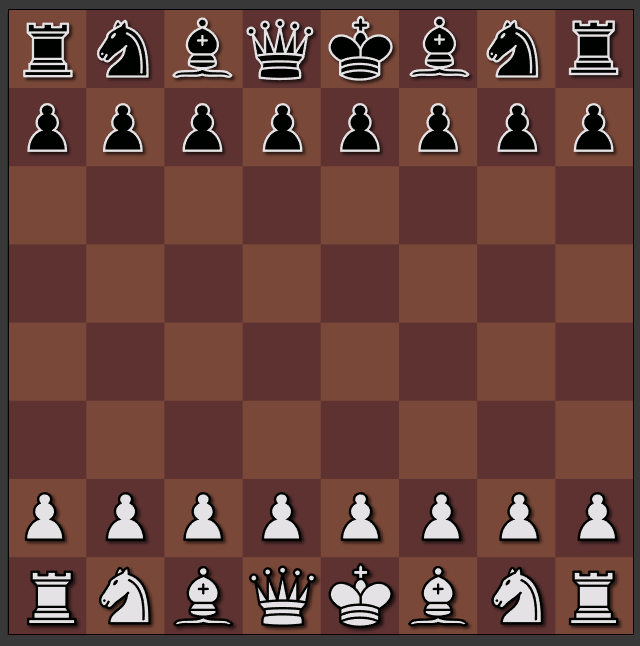
\includegraphics[scale=0.6]{image5.png} \\
    	\textit{This illustration and pieces in section 5 were made by: (JohnPablok, 2018)}
    \end{center}
    
    \section{Our GUI concept}
    \begin{center}
        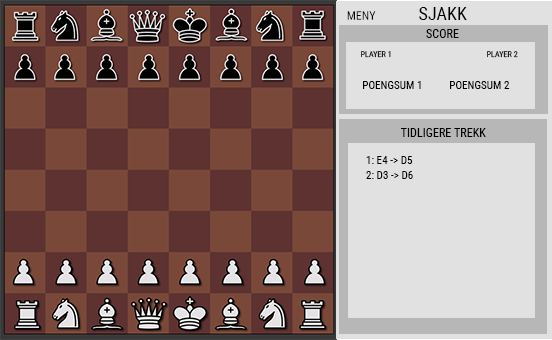
\includegraphics[scale=0.6]{mockup_chess.png}
    \end{center}

    
    
    \section{An outline of the rules and key features of the game}
    \noindent
    Chess is a game between two players  -- White and Black -- who alternate turns. White always moves first. Players move one piece at a time until one player captures the enemy's king.  Chess uses 6 pieces and each of them moves in a specific way. However all pieces share some common traits. No piece is allowed to move to a place that is already taken by a friendly piece. If the piece lands on a square occupied by an enemy piece, that square is captured and the enemies piece is removed from the board. board.Pieces are not allowed to jump over other pieces, with the exception of the knight. (Scima, 2017)\\
A game is won when the opponents king is set in checkmate. This means the king is threatened by a piece, has nowhere
safe to move, and no way of removing or blocking the threatening pieces.\\

\vspace{20mm}
\section{Types of pieces:}
\begin{itemize}

    
    \item \textbf{The rook} - looks like a small tower. It moves in a straight line horizontally or vertically for any number of squares. \\
	  \begin{center}
    	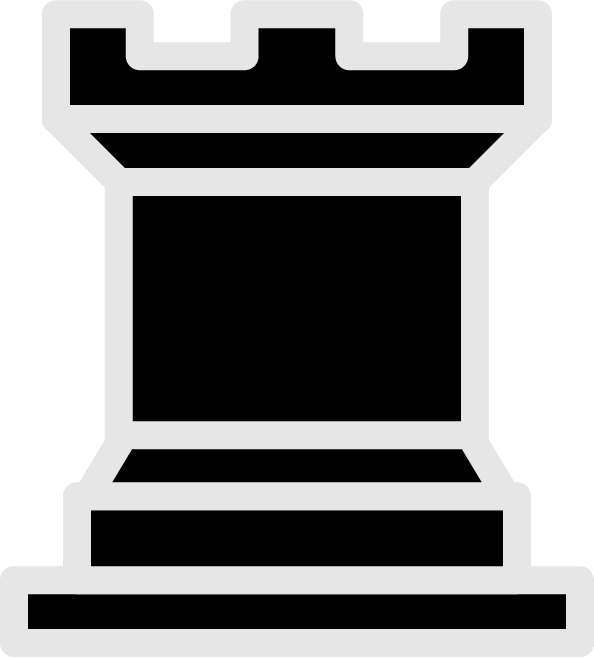
\includegraphics[scale=0.1]{image3.png}
    	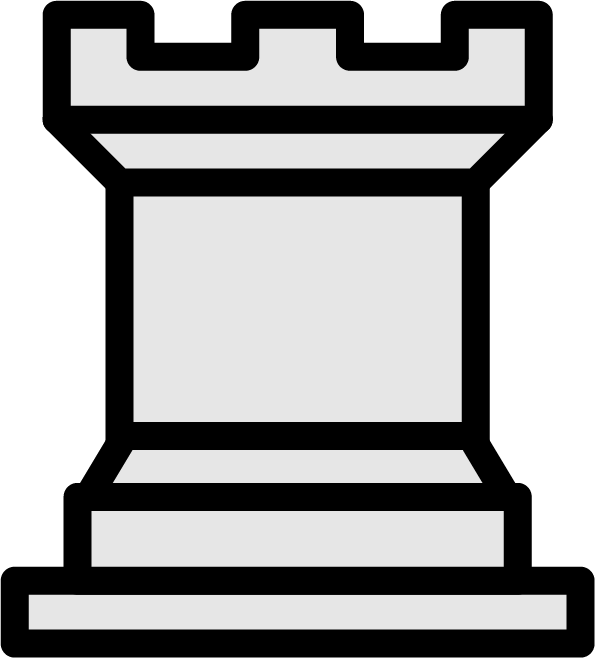
\includegraphics[scale=0.1]{image7.png}
    \end{center}
    
    \item \textbf{The bishop} - moves in a straight line diagonally for any number of squares.\\
    \begin{center}
    	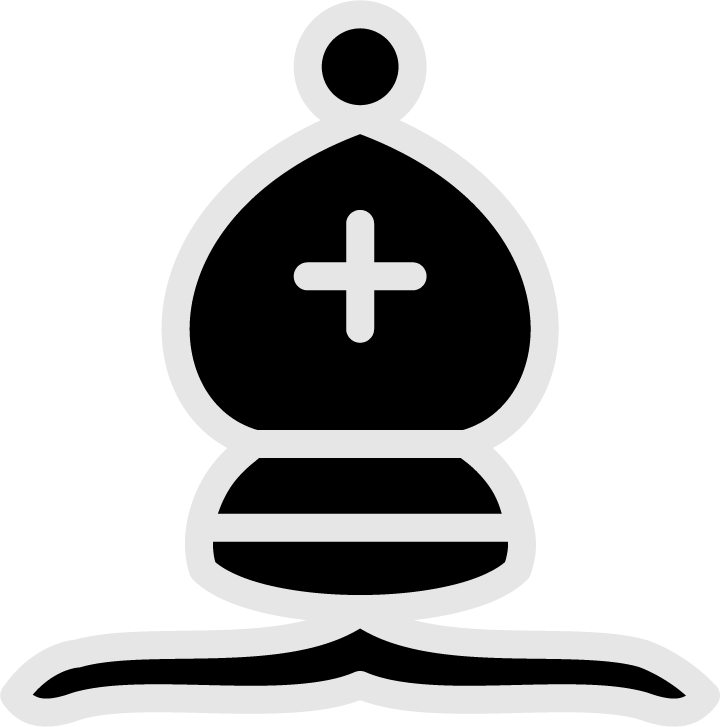
\includegraphics[scale=0.1]{image1.png}
    	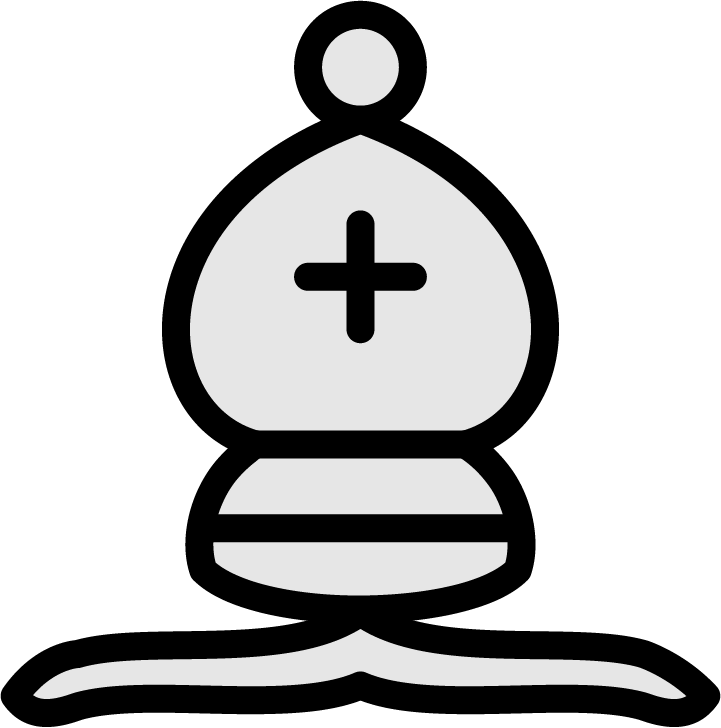
\includegraphics[scale=0.1]{image16.png}
    \end{center}
    
    \item \textbf{The queen} - looks like a queens crown. Most powerful piece in the game. Moves in a straight line either horizontally, vertically or diagonally for any number of squares.\\
    \begin{center}
    	
\includegraphics[scale=0.1]{image14.png}
    	
\includegraphics[scale=0.1]{image4.png}
    \end{center}

    \item \textbf{The king} - looks like a kings crown. Can also move in any direction, but it can only move one square at a time. \\
    \begin{center}
    	
\includegraphics[scale=0.1]{image9.png}
    	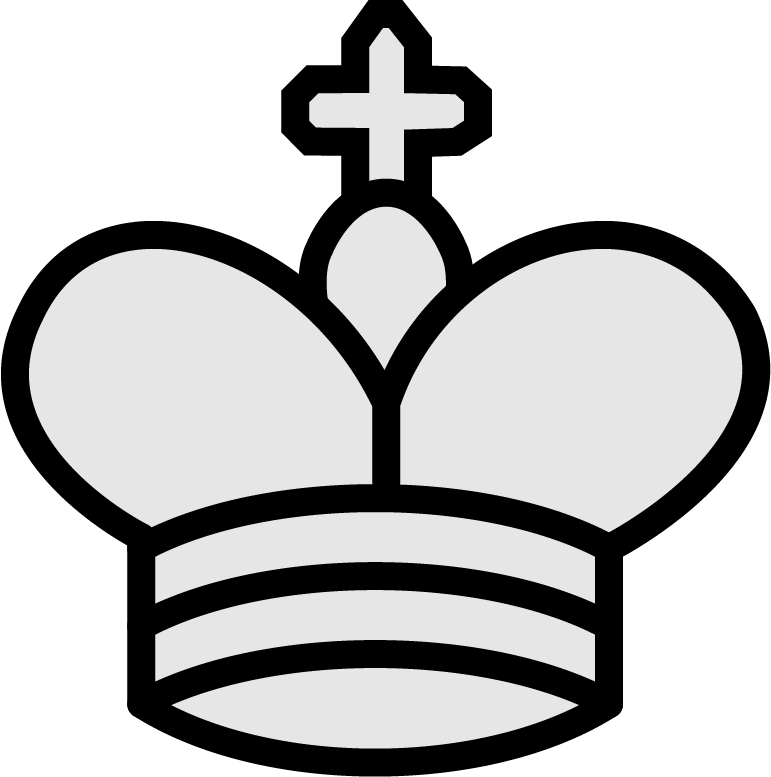
\includegraphics[scale=0.1]{image8.png}
    \end{center}

    \item \textbf{The knight} - looks like a horse. This piece moves in a irregular L-shaped pattern. The knight moves two squares horizontally or vertically, then turns at the right angle to move one more square. It can jump over pieces, but it does not capture the pieces it jumps over. It will only capture the square it lands on. \\
    \begin{center}
    	
\includegraphics[scale=0.1]{image13.png}
    	
\includegraphics[scale=0.1]{image10.png}
    \end{center}
    
    \item \textbf{Pawns} - the weakest piece in the game. The pawn can only move forward, not backward or sideways. They move only one square directly forwards. However they cannot capture a square this way. The pawns can only capture the square forward diagonally. Additionally, the pawns that are on the starting square have the opportunity to move two squares directly forward.\\
    \begin{center}
    	
\includegraphics[scale=0.1]{image2.png}
    	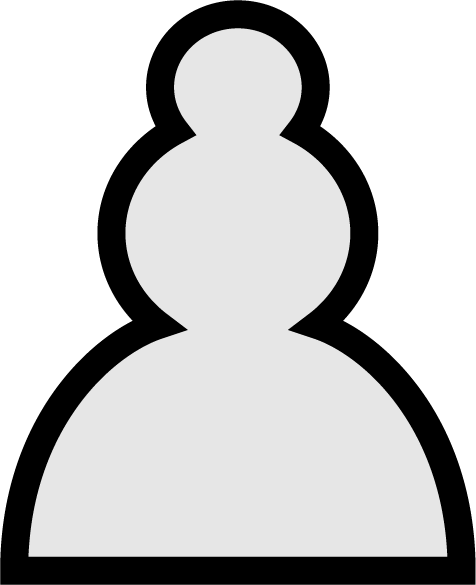
\includegraphics[scale=0.1]{image6.png}
    \end{center}
\end{itemize}

\section{Special rules:}
\begin{itemize}

\item \textbf{Check} - a player’s king is “in check” when it can be attacked by an opponent’s piece. If the king is in check, the player must find a way to prevent the king from being captured.

\item \textbf{Castling} - The rule is used to improve kings safety.  This is the only rule that allows two pieces move at the same time - the king and a rook. It can only happen if all of the following conditions are present.

\begin{itemize}
   \item Neither the king or the rook has yet been moved during the game. If either of the pieces have been moved, this rule is not allowed. 
   \item All of the squares between the king and the rook must be empty.
   \item The king must not be in check, nor can castling move the king through a square where it would be check. 
   \end{itemize}

\item \textbf{Pawn promotion} - pawns are the weakest pieces of chess, but they can potentially become much stronger. If the pawn manages to get to the other side of the board, the pawn must be promoted to any piece the player chooses, except the king. 

\item \textbf{En passant} - french for “in passing”. If a pawn moves two squares on its first move and by doing so lands on the side of an enemy pawn (jumping past the enemy’s pawns ability to capture it). The enemy pawn has the option to capture the pawn as it passes by. This special move must be done immediately after the first pawn has moved past. Otherwise the option is no longer available. 

\item \textbf{Threefold repetition rule} - The game will draw if the exact same boardstate occurs three times. The repeated
positions do not need to occus in succession. The idea behind the rule is that if the boardstate occurs three times, no progress
is being made. 
\end{itemize}

\section{References}
\begin{itemize}
\item JohnPablok (2018) Chess board.Pieces and board.Board squares [Internet]. \\
	  Available from: \textit{https://opengameart.org/content/chess-pieces-and-board-squares} \\
	  Read: 21.february 2018\\
	  License: \textit{https://creativecommons.org/licenses/by-sa/3.0/}
\end{itemize}
\end{document}
